\pagenumbering{roman}

\begin{titlepage}
\begin{center}
\Huge{
	{\textbf{\titlecap \ipapertype}}
}
\end{center}
\newpage

\thispagestyle{empty}

\hfill 
\includegraphics[height=1.5cm]{images/FHSLogo.pdf}

\vspace*{2cm}

\Large{
\MakeUppercase\ititle

\vspace*{1cm}

\MakeSentenceCase{\ipapertype}~\tattainment

\vspace*{0.5cm}

\textit{\tdegree}
}


\vspace*{1.5cm}
{\large
\tauthor: \iauthor
}
\vfill

{\normalsize
\tsubmitted

\vspace*{1cm}

\begin{tabbing}
\hspace*{1.4in}\=\kill
\texamined: \> \ \isupervisor~(\tsupervisor)
% uncomment the following line for an optional second supervisor:
%\\          \> \ Dr. Tommy Thompson~(2. \tsupervisor)
\end{tabbing}

\vfill
\selectlanguage{ngerman}
Salzburg, \today
\selectlanguage{english}
}
\end{titlepage}

\setcounter{page}{1}

\isection{Eidesstattliche Erklärung}

Hiermit versichere ich, Vorname Familienname, geboren am {\bf Tag.Monat.Jahr} in {\bf Ort}, dass ich die Grundsätze wissenschaftlichen Arbeitens nach bestem Wissen und Gewissen eingehalten habe und die vorliegende Masterarbeit von mir selbstständig verfasst wurde. Zur Erstellung wurden von mir keine anderen als die angegebenen Quellen und Hilfsmittel verwendet. 

Ich versichere, dass ich die Masterarbeit weder im In- noch Ausland bisher in irgendeiner Form als Prüfungsarbeit vorgelegt habe und dass diese Arbeit mit der den BegutachterInnen vorgelegten Arbeit übereinstimmt.


\vspace*{3cm}

{\bf Salzburg}, am {\bf \today}


\hfill


Unterschrift

\vspace*{1cm}

\hfill \imatrikel\hspace*{1cm}\newline
$\overline{\text{Vorname Familienname}}$ \hfill	$\overline{\text{Personenkennzeichen}}$

\selectlanguage{ngerman}

\section*{Kurzfassung}
\vspace{0.5cm}

Deutsche Zusammenfassung ...

... ungefähr 200 Worte ...

\textbf{Schlagwörter:}\\
\textit{Keyword 1, Keyword 2}


\selectlanguage{english}


\isection{Abstract}

There has never been such a quantity of data available in history and the global amount of information has never grown so strong and continuous. Processing and analysis of data garners increased economic and scientific interest. Finding useful and usable information in such a heap of data is a tedious and time consuming task. Visualisations are a handy tool to explore unknown data. However, there are many different types of visualisations possible to achieve one objective. Choosing the best visual representation is often based on the domain knowledge of the creator. They are often unaware of the strengths and weaknesses of each type of visualisation and therefore also its use cases. Thus, this thesis presents a way of using animated transitions between different visual representations to help pointing out advantages and disadvantages of these. The implemented application trying to achieve this is publicly available and its usefulness is tested with a user study.


\textbf{Keywords:}\\
\textit{Keyword 1, Keyword 2}

\clearpage
\tableofcontents
% \addtocontents{toc}{\protect\pagebreak}

\clearpage
\isection{List of Abbreviations}
\listofabbreviations
\clearpage

\setcounter{page}{1}
\pagenumbering{arabic}

\section{Introduction}

\bigskip

\ac{ai} is defined as the ability of machines to act and think similar to humans \iacite[29]{millington.2009}. Usually the behaviour of an \ac{ai} is abstracted by the game designer and then implemented. This way they are solving the specific problem in the intended way. Most often those \acp{ai} are inflexible and tend to fail to perform in different domains.

\section{Methods}

\section{Results}

\section{Discussion}

\section{Outlook}



\section{Related Work}
The first part of this chapter provides an overview of the related work in the field of
Information Visualization. First general methods, which are important for visualizations of heterogeneous data in this area of application, are described. This rather high level discussion is followed by a more specialized view on map-based visualizations and transitions in visualizations. The combination of these two emerging research areas leads to the application of map-based visualizations with transitions between them. Finally the current state in the domain of map-based visualization is summarized and potential improvements are identified.

\subsection{Geovisualization methods}
Visualization as a term is fist mentioned 1953 in the cartographic literature, in an article by University of Chicago geographer Allen K. Philbrick. 1987 new developments in the field of computer science prompted the National Science Foundation to redefine the term. The report of the redifinition placed visualization at the convergence of computer graphics, image processing, computer vision, computer-aided design, signal processing, and user interface studies \iacite{mccormick:1987}. Visualization now also emphasizes the knowledge creation and hypothesis generation aspects of \ac{scivis}.

In the early 1980s, a french graphic theorist named Jacques Bertin set a milestone in the area of scientific research. Based on his work in this \ac{geovis} developed as a field of research. His work shows a strong focus in the research of the potential for the use of dynamic visual displays as prompts for scientific insight and of the methods through which dynamic visual displays might leverage perceptual cognitive processes to facilitate scientific thinking \iacite{maceachren:2004}.

As already mentioned, \ac{geovis} is closely related to the fields of \ac{scivis} and also \ac{infovis} and emphasizes knowledge construction over knowledge storage or information transmission \iacite{maceachren:1997}. However \ac{infovis} needs to be strictly differentiated from \ac{scivis}. \ac{infovis} deals with abstract data like for example movies in a movie database whereas \ac{scivis} operates on real-world data with spatial character.

\ac{geovis} also contributes significantly to other related fields such as \ac{scivis} and also \ac{infovis}. Owing to its roots in cartography, \ac{geovis} contributes to these other fields by way of the map metaphor, which "[\ldots] has been widely used to visualize non-geographic information in the domains of information visualization and domain knowledge visualization" \iacite{Jiang2005}. It emphasizes knowledge construction over knowledge storage or information transmission \iacite{maceachren:1997}. However \ac{infovis} needs to be strictly differentiated from \ac{scivis}. \ac{infovis} deals with abstract data like for example movies in a movie database whereas \ac{scivis} operates on real-world data with spatial character.

These kind of visualizations are also already used in practical applications. The following list shows some summarized examples of these applications:
\begin{description}

\item[Urban Planning] \hfill \\
Urbanists use \ac{geovis} to "[\ldots] model environmental interests and policy concerns of the general public" \iacite{Jiang2003}. \citeauthor{Jiang2003} also mention two examples, in which "[\ldots] 3D photorealistic representations are used to show urban redevelopment and dynamic computer simulations are used to show possible pollution diffusion over the next few years".

\citeauthor{Jiang2003} also describe that the widespread use of the internet by the general public allows collaborative planning to be conducted in both centralised and decentralised manner. The former way of planning in committee rooms or computer facility rooms can be extended with a decentralised web platform. This platform would lead to increased parcitipation by the public because
\begin{enumerate}
\item the internet already integrates various interactive and proactive techniques and
\item is time and place independent.
\end{enumerate}


\end{description}


Traditional, static maps have a limited exploratory capability. The graphical representations are inextricably linked to the geographical information beneath. \ac{gis} and \ac{geovis} allow for more interactive maps. Both of them have the ability to extend the basic layer of a map with user-experience abilities like for example zooming in or out and to change the visual appearance of the map \iacite{Jiang2003}.
\section{Methods}
The first part of this chapter provides an overview of the related work in the field of
thematic cartography. This topic is going to be combined with basic principles of visualizations and visual design principles. Afterwards, \ac{GeoVis} is explained from a practical point of view and the connections to close related fields are made. This rather high level discussion is followed by a more specialized view on four different map-based visualizations. The combination of thematic cartography and interaction leads to the next sections, where different interaction approaches are explained in detail. Finally the current state in the domain of map-based visualization tools is analysed, summarized and potential improvements are identified.

\subsection{Thematic Cartography}
\label{s:cartography}
The origin of cartography lays far back in the history of visualization as shown in chapter \ref{s:history} on page \pageref{s:history}. Today's understanding of modern cartography began in the late 18\textsuperscript{th} century with the attempt to show more than one attribute in a map. \citeauthor{Longley2005} say, that topography has long been understood as an important aspect of war strategy. Battles and wars could be decided on the information of the topology. A commander had to position his units wisely in order to exploit all geographical circumstances and thus have an advantage over his opponent \iacite{Longley2005}.
in the middle of the 20\textsuperscript{th} century, the Soviets, Fascist Italy and Nazi Germany all used map to foster national pride. This could furthermore be used to justify their expansionism \iacite{Crampton2015}.
Today, national organisations produce a variety of maps for different reasons with a very high focus of map accuracy (see chapter \ref{s:map-accuracy} on page \pageref{s:map-accuracy} for more information) and transmittal of relvant information.

The field of cartography can be divided into two major subcategories:
\begin{enumerate}
\ditem{General cartography} is associated with maps that are constructed for commonalty. These type of maps often contain a variety of features and display many reference and location systems. An abstract definition of general maps is that those kind of maps show the variety of phenomena of either geological, geographical or policital nature together \iacite{Thrower2008}.

\ditem{Thematic cartography} focuses on a specific subject area, often called theme. Thus it involves maps which emphasize spatial variation of geographic distributions. \citeauthor{BartzPetchenik1979} describes thematic maps compared to general (or reference) maps as "in place, about space". She says, that the a general map is characterized by the fact that it shows you where something is in space, according to the example. However, thematic maps will tell a story about that specific place \iacite{BartzPetchenik1979}.
In order to make a connection to the abstract definition \citeauthor{Thrower2008} made for general maps, thematic maps could be described as follows:
Those kind of maps (thematic) use the base data only as points of references. Base data could be coastlines, boundaries and places. Phenomena of all kind are being mapped onto the reference \iacite{Thrower2008}.
\end{enumerate}

The following sections in this chapter should provide general knowledge about different types of maps, scaling, projecting, generalization and symbolization and accuracy. This knowledge is needed in order to understand the implementation of the partical part of this thesis.

\subsubsection{Methods of thematic maps}
The two major categories of cartography are general cartography and thematic cartography, which are introduced in chapter \ref{s:cartography} on page \pageref{s:cartography}. This categorization can be directly mapped from cartography to maps. The main objective of this chapter is to give an overview of different thematic maps and their usage. These maps can be subdivided into univariate and multivariate maps.

\subsubsubsection{Univariate Thematic Map Types}
Univariate maps are only dependent on one variable, except for the map variables like latitude and longitude and suchlike.

\sectionparagraph{Dot density map}
\input{chapters/methods/cartography/dot}

\sectionparagraph{Graduated symbol or proportional symbol map}
\input{chapters/methods/cartography/psm}

\sectionparagraph{Choropleth map}
\input{chapters/methods/cartography/choropleth}
\label{s:choropleth}

\subsubsubsection{Multivariate Thematic Map Types}

\subsubsection{Map Scale}
\subsubsection{Map Projections}
\subsubsection{Map Generalization}
\subsubsection{Symbolization}
\subsubsection{Map Accuracy}
\label{s:map-accuracy}


\subsection{Geographic Visualization}
Chapter \ref{s:definitions-types} on page \pageref{s:definitions-types} already defines \ac{GeoVis}. It is closely related to \ac{InfoVis} and \ac{SciVis} and emphasises knowledge construction over knowledge storage or information transmission \iacite{maceachren:1997}. Owing to its roots in cartography, \ac{GeoVis} contributes to its related fields by way of the map metaphor, which "[\ldots] has been widely used to visualize non-geographic information in the domains of information visualization and domain knowledge visualization" \iacite{Jiang2005}.
In short, the thesis uses the term \ac{GeoVis} as a hypernym for the combination of exploratory data analysis, \ac{InfoVis}, \ac{SciVis}, thematic cartography and visual analytics.

\ac{GeoVis} are superior to traditional, static maps because they are not limited to exploration capabilities. They allow more interaction in maps, due to the ability of extending the basic layer of the map with user-experience abilities like zooming to change the visual appearance \iacite{Jiang2003}. These kinds of visualisations are also used in practical applications which are briefly outlined in this chapter.

\begin{description}

\item[Urban Planning] \hfill \\
Urbanists use \ac{GeoVis} to "[\ldots] model environmental interests and policy concerns of the general public" \iacite{Jiang2003}. \citeauthor{Jiang2003} also mention two examples, in which "[\ldots] 3D photorealistic representations are used to show urban redevelopment and dynamic computer simulations are used to show possible pollution diffusion over the next few years".
\citeauthor{Jiang2003} also describe that the widespread use of the internet by the general public impacts collaborative planning. The former way of planning in committee rooms or computer facility rooms can now be extended with a decentralised web platform. The use of the internet features two important aspects of planning:
\begin{enumerate*}
\item it already integrates various interactive and proactive techniques and
\item it is time and place independent.
\end{enumerate*}

\item[Environmental Studies] \hfill \\
\citeauthor{Danado2005} describe a system that is capable of simulating and visualising environmental processes collaboratively. In addition, the system has the ability to retrieve information while moving in real time. Thus each user can impact the simulation by adding or removing information to or from the model. The system also reacts on the changes the users made, therefore making it possible to explore a complex set of environmental data, affecting it with different actions and determine a best fit \iacite{Danado2005}.

\item[Forestry] \hfill \\
\citeauthor{Andrienko2007} present a system to visualise a large set of spatio-temporal data related to european forests. The innovative approach of this system is given by the interaction. Non-experts can change parameters in the system and explore the results. Furthermore \citeauthor{Andrienko2007} state their approach "[\ldots] uncovers a range of fundamental issues relevant to the broad field of \ac{GeoVis} and \ac{InfoVis} research \iacite{Andrienko2007}."

\citeauthor{Andrienko2007} also cited the two major problems as
\begin{enumerate}
\item the inability of the geovisualisers to convince the foresters of the efficiency of \ac{GeoVis} in their work and
\item the foresters' misgivings over the dataset's accessibility to non-experts engaging in "uncontrolled exploration".
\end{enumerate}

\item[Telecommunication] \hfill \\
\ac{GeoVis} are also very helpful in the area of telecommunication. Telegeography\footnote{https://www.telegeography.com/}, as an example for a company in that specific area, has an interactive submarine cable map. Figure \ref{fig:both-submarines} on page \pageref{fig:both-submarines} features an overview of this map (see figure \ref{fig:submarine}) and the interactivity (see figure \ref{fig:submarine-interactive}) which gives more information to the cable’s profile, including the cable’s name, ready-for-service date, length, owners, website, and landing points.

\begin{figure}[!htb]
  \captionsetup[subfigure]{justification=centering}
  \centering
  \begin{subfigure}[b]{0.4\textwidth}
    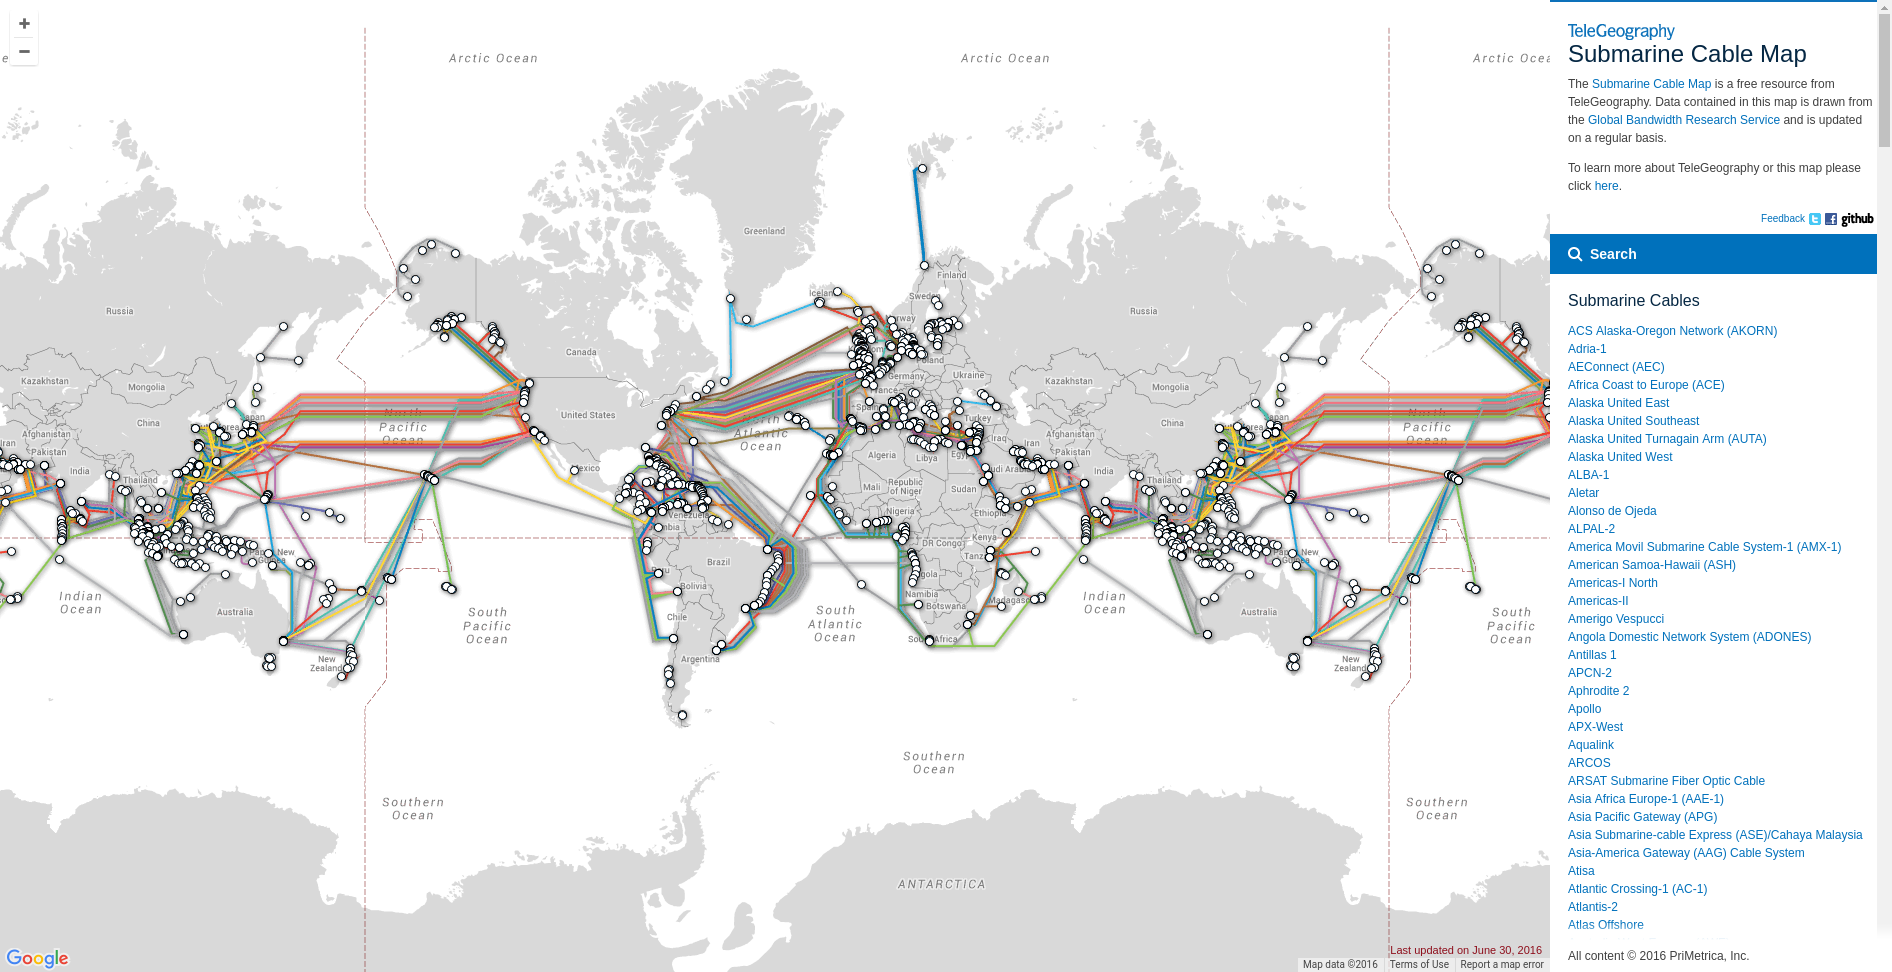
\includegraphics[width=\textwidth]{images/geovis/submarine.png}
    \caption[Overview of the submarine cable map]{Overview of the submarine cable map}
    \label{fig:submarine}
  \end{subfigure}
  \hfill
  \begin{subfigure}[b]{0.4\textwidth}
    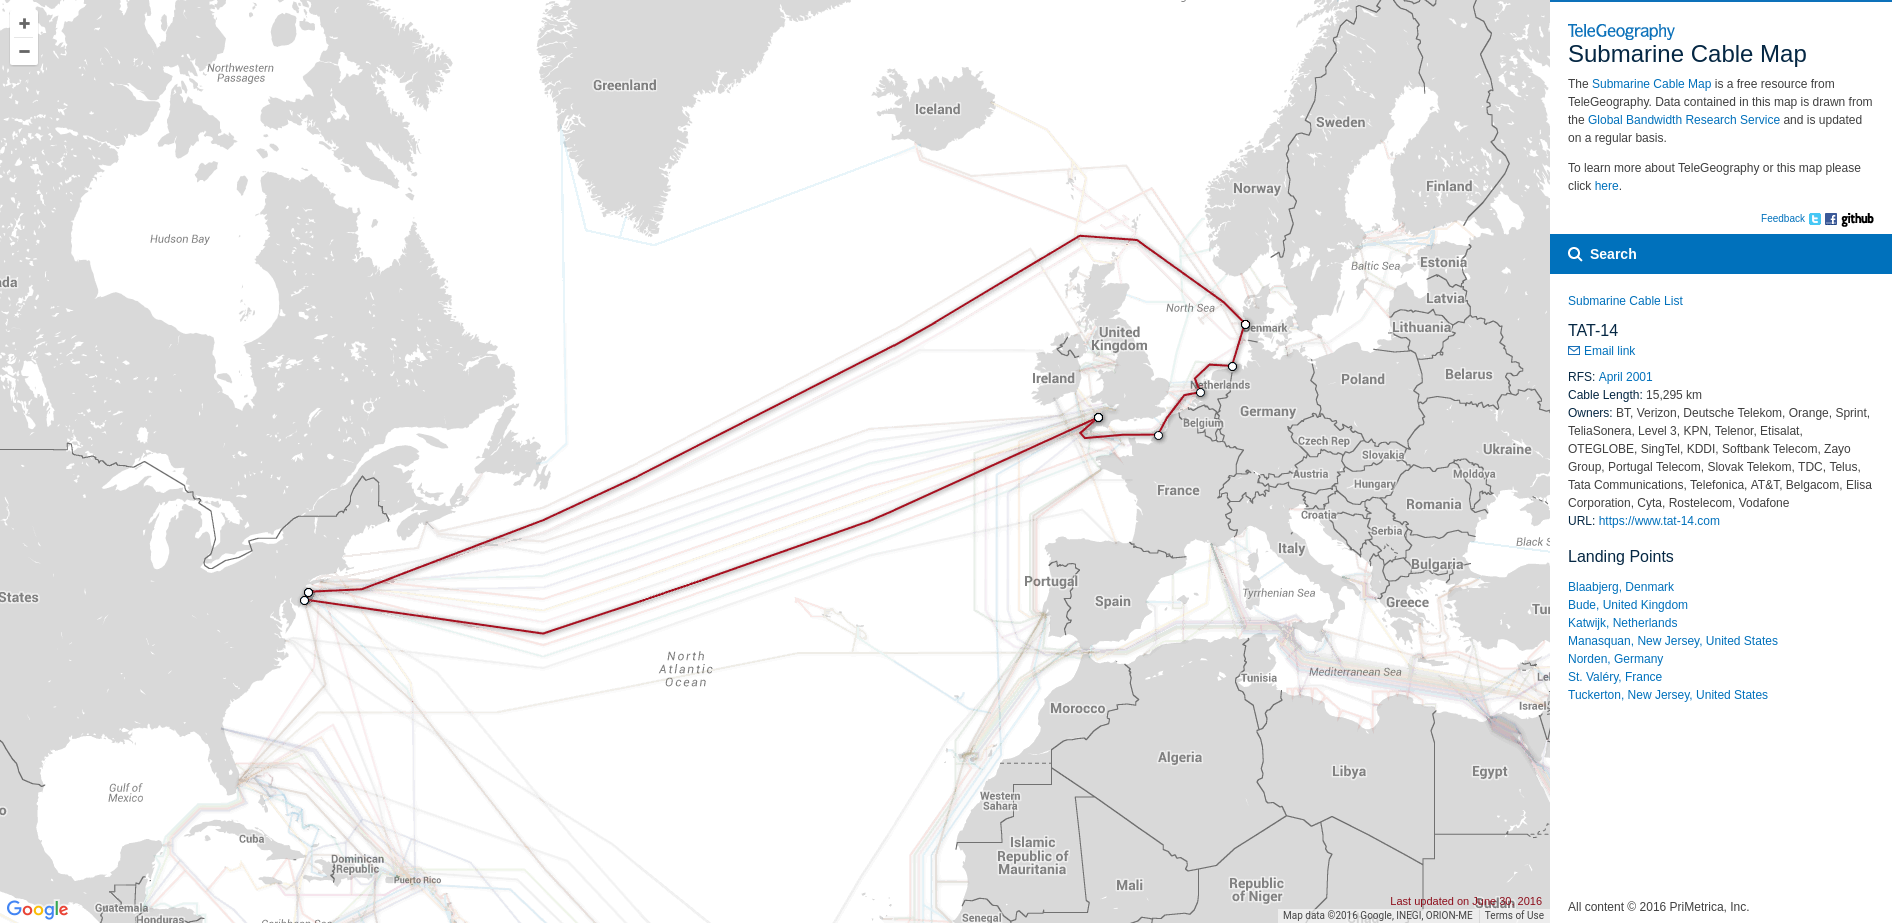
\includegraphics[width=\textwidth]{images/geovis/submarine-interactive.png}
    \caption[Interactivity of the submarine cable map]{Interactivity of the submarine cable map}
    \label{fig:submarine-interactive}
  \end{subfigure}
    \caption[
        TeleGeography’s free interactive submarine cable map, Urldate: 07.2016 \newline
    \small\texttt{\url{http://www.submarinecablemap.com/}}
    ]{TeleGeography’s free interactive submarine cable map}
  \label{fig:both-submarines}
\end{figure}

\item[E-commerce] \hfill \\
\ac{GeoVis} can be very useful in analysing data provided by e-commerce shops if they track orders-behaviour of their customers with some kind of geographical information. If such data is available and provided, it is possible to easily visualise the target group of a company on a map and therefore create knowledge and allow for generating hypothesis i.e. the next region for expansion.

\end{description}

\subsection{Interaction in visualizations}
\label{s:interaction}
When designing maps, there is one important distinction: designing maps for print versus the internet. For the first case, the design is for map readers, whereas for the latter case, it is for map users. The difference between readers and users lays in the interaction. This chapter focuses on a map designed for the internet and therefore allowing a lot more interaction. Users do not only interact but also manipulate web maps. Interaction for print maps would be moving a paper map closer or further away to one's eyes, or trim specific parts with scissors and so forth. The weakness of this kind of interaction is that the data on the map stays the same. However, zooming, selecting and moving a map on the internet actually allows for adapting the data shown \iacite{Muehlenhaus2014}.

As already mentioned in chapter \ref{s:definitions-types} on page \pageref{s:definitions-types}, \citeauthor{Shneiderman1996} published an often cited mantra \iacite{Shneiderman1996}:
\begin{quote}
"Overview first, zoom and filter, then details on demand."
\end{quote}

% MISSING BOOK: Information Visualization: Design for Interaction Spence 2007
% This mantra can also be used as a guideline for creating web maps with interaction.
% % Spence2007
% introduces a so called action cycle, which models an interactive exploration process of data. Small datasets, as well as complex and dynamic data can make use of this process in order to properly implement and integrate interaction.

% TODO - CHECK IF ENOUGH WORDS

The first part of this chapter will introduce some basic interaction methods and concepts. The second part will build upon the knowledge of the first part and maps the basic concepts to today's implementations with the focus on interaction with thematic maps.

\subsubsection{Overview First, Focus \& Context}
A natural way according to the mantra presented by \citeauthor{Shneiderman1996} to visualise a dataset is to start with an overview. This supports the user's understanding of the complexity and size of the whole dataset. However giving an overview first is also dependant on the dataset. Imagine a \ac{GIS} like OpenStreetMap\footnote{See \href{https://www.openstreetmap.org}{https://www.openstreetmap.org}} would show random location, e.g. a valley with a lot of detail as a starting point. There are two contrary use cases where such a starting point would make sense or not.
\begin{enumerate}
\item If the dataset the map is based on only contains data of that specific ``random'' valley shown, it definitely makes sense to only show that valley. The dataset does not contain information about all valleys, therefore making it unnecessary to show the whole map of the earth as an overview first.
\item The use case mentioned already, implicitly explains a bad use case of a random starting point. If a dataset inheres structure, like a whole map of the world, it is not useful to start at a specific location, therefore showing an overview of the earth first makes more sense.
\end{enumerate}

Focus and context describes a concept that puts a specific part of dataset, called subset, in focus while still showing an overview of the other part. One example implementation of this concept are fisheye views, originally developed by \citeauthor{Furnas:1986} \iacite{Furnas:1986}. Figure \ref{fig:focus} on page \pageref{fig:focus} shows a modern implementation of the focus and context concept based on a fisheye view. The focus in this Figure is set somewhere between the blue and orange circle in the middle of the Figure. This part is magnified as one can see on the circle size, while the ones further away are smaller and a little distorted.

\begin{figure}[!htb]
\centering
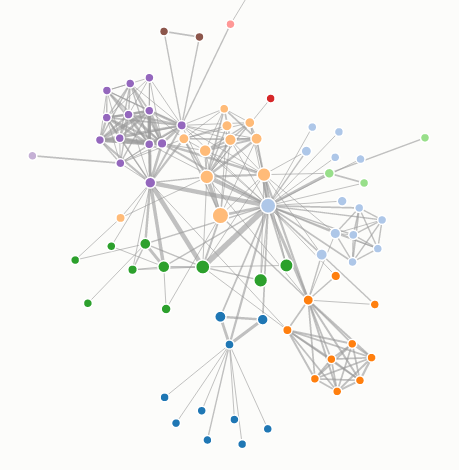
\includegraphics[height=5cm,keepaspectratio]{images/methods/interaction/focus.png}
\caption[
    The focus and context concept based implemented with a fisheye view, Urldate: 07.2016 \newline
    \small\texttt{\url{https://bost.ocks.org/mike/fisheye/}}.
]{The focus and context concept implemented with a fisheye view. The blue node in the center of the Figure and the yellow node left to it are bigger compared to the other ones. This is due to the magnification of this part.}
\label{fig:focus}
\end{figure}

\citeauthor{Kosara2003} categorise the aforementioned method as distortion-oriented \iacite{Kosara2003}. Other techniques they list are summarised below:
\newpage
\begin{description}
\item[Overview methods] show the context in a separate layer in the same place \iacite{Kosara2003}.
\item[Filtering] shows additional information of particular subparts e.g. with a magic lens. They provide an object of any shape that can move freely. The area it covers is shown with more information \iacite{Bier:1993}.
\item[In-Place techniques] are similar to filtering without the requirement of a lens. The implementation of the technique points out information to the user, e.g. by highlighting. The program can also take the initiative and point the user to interesting data \iacite{Kosara2003}.
\end{description}


\subsubsection{Details on Demand}
Showing detailed information upon interaction on a dot map based on a dataset with 10000 data items describes the concept of showing details on demand. It would be infeasible to show details on all entries, as the screen-space is limited. Even with unlimited screen-space it, would drastically worsen the readability of the map. \citeauthor{Ahlberg:1996} explains one possible way of implementing this concept. His approach is to only show objects that match certain criteria and are therefore likely of interest to the user. However, the user needs to start this task first with some kind of interaction, e.g. clicking on a visual object of a specific type. The additional information is then shown in a pop-up window \iacite{Ahlberg:1996}.



\subsubsection{Multiple Views, Linking \& Brushing}
\label{s:linking-brushing}
Multiple view systems are defined by using several views on the same dataset, but with different aspects of it for each visualization. Practical applications of all kinds make use of such a system, e.g. \ac{CAD} and \ac{GIS}. Even though the possibility of using multiple views on the same dataset is trivial, the implementation and necessary amount of interaction is not \iacite{Kosara2003}.

\citeauthor{Baldonado2000} present four design rules wheter or not multiple view systems are appropriate for the specific task \iacite{Baldonado2000}:

\begin{enumerate}

\ditem{Diversity} \hfill \\
If the given dataset consists of attributes with different types, multiple levels of abstraction, and so forth, a multiple view system can be created. A single view would be overloaded with the given dataset because of the significant cognitive overhead created. The user would need to simultaneously comprehend and assimilate a multitude of diverse data.

\ditem{Complementarity} \hfill \\
Multiple view systems support visual comparability. They should be used if showing correlations and/or disparities is important, because they leverage multiple perceptual capabilities to improve understanding of relations among views.

\ditem{Decomposition} \hfill \\
Showing different attributes at the same time provides insight in different dimensions. This rule is related to the "divide and conquer" principle: the amount of data a user needs to consider at one time is reduced, thus aiding memory.

\ditem{Parsimony} \hfill \\
Multiple views build upon the cost of switching context and increasing complexity. The learning cost of a user, aswell as computational and display space costs of several views must be justifiable.

\end{enumerate}

Multiple view systems are often used for focus and zoom, e.g. for showing the focus and contex in seperate windows. \citeauthor{Robert:1998} describe a system based on this concept \iacite{Robert:1998}.

\citeauthor{Martin:1995} describe brushing as the process of selecting specific data items or groups of items to highlight them \iacite{Martin:1995}. Usually this process is initiated by directly interacting with the view using the mouse. Two possible manual interactions are opening a rectangular region of interest or clicking on a specific data items. It can also be accomplished without interacting with the visualization itself by using sliders, select-boxes or even complex means like selecting a cluster \iacite{Kosara2003}.

However, using the brushing technique is not sufficient when exploring complex data efficiently. Linking describes the concept of exchanging information about which points are brushed. This concept is essential when using brushing and multiple view systems together. With this combination, a user can easily see the same points brushed in different views on the data \iacite{Kosara2003}.



\subsubsection{Animations and Transitions}
In order to understand transition referring to visualizations, it is important to point out the difference between transition and animation. Even though these two terms are often substituting each other, they follow two different concepts \iacite{Muehlenhaus2014}:

According to the Merriam Webster Online Dictionary\footnote{See \href{http://www.merriam-webster.com/}{Merriam Webster Dictionary}} an animation is a way of making a movie by using a series of drawings, computer graphics or photographs that are slightly different from one another and that when viewed quickly one after another create the appearance of movement. Transition, however, is a movement, development, or evolution from one form, stage, or style to another.

With these definitions, it is easy to distinguish the two terms. Animation is the process of making any kind of movement visible to a user, whereas transitions in visualizations make use of animations to show e.g. the change of visual appearance.

\citeauthor{Thrower1959} was the first one to combine the research fields of cartography with animation. He describes the process of bringing e.g. population growth with animation on a map \iacite{Thrower1959}. However, animated cartography remained a bit of an oddity that was experimented with. This fact could not be changed even with the rise of the household \ac{PC}. Nonetheless, the mass adoption of the internet could counteract the rare usage of map animation \iacite{Muehlenhaus2014}.

This chapter furthermore describes considerations when designing animated maps. Animation can basicly be broken down into two broad types:

\begin{enumerate}
\ditem{Stop-Frame Animation} \hfill \\
This type of animation is also known as stop motion. Every frame of this type of animation is designed separately. After many pictures and movements are made, all pictures are in the order they were taken. The rate of change for each picture heavily influences the cognition of the animation \iacite{Faroudja1991}.
\ditem{Tweening} \hfill \\
    This term bears its name from the word "betweening". It describes the process of interpolating movement between key frames, thus creating smoother animations compared to the stop-frame method \iacite{Muehlenhaus2014}.
\end{enumerate}

\citeauthor{DiBiase1992} identified three new visual variables dealing specifically with animation \iacite{DiBiase1992}:

\begin{enumerate}

\ditem{Duration} defines the temporal length of how long a particular frame in an animation is shown. Imagine a dataset containing decennial census of population data and an animation set to 24 frames per second. To give each map user the ability to conceive each decade, it is needed to show it at least for some seconds. For the sake of convenience a duration of 2 seconds is assumed to be enough. Therefore, it is needed to show each decennial census data for 48 frames, resulting in a 2 second duration \iacite{Muehlenhaus2014}.

\ditem{Rate of Change} represents how quickly an image is morphed into the next attribute. In general, it denotes the magnitude of an attribute divided by the duration. This basically means, that it is needed to know how much the animated image being represented changes from frame to frame \iacite{Muehlenhaus2014}.

\ditem{Order}
Rather than animating data in the order they are given, they can be reorganized first by a specific attribute. For example, one could show all countries with a high population first, before showing small ones \iacite{Muehlenhaus2014}.

\end{enumerate}

\citeauthor{Muehlenhaus2014} also mentions differnt types of map animations. He says weather forecasts are the most common use case for map animations. Thus deriving the term temporal animation for this kind of animation seems appropriate. Albeit showing change over time seems trivial, people do not always interpret the resulting animation accurately. He suggests the use of temporal animations for showing broad patterns of change in a dataset. However, the animation should either show broad changes in a small scale or detailed changes in a large scale. This heavily impacts the user's perception and interpretation of the animation, including "change blindness". This means, that obvious changes in a map are missed due to focusing something else in the map. In order to combat the problem of change blindness, he \citeauthor{Muehlenhaus2014} names three different design principles \iacite{Muehlenhaus2014}:

\begin{enumerate}

\item \textbf{Animation duration} should be kept short in order to not overwhelm a user's short-term memory. Temporal animations should not take longer than 30 seconds to a minute, especially when showing changes in data, which are not narrative in nature. If this principle is ignored, data retention will be nullified \iacite{Muehlenhaus2014}.

\item \textbf{Data simplification} denotes the amount of animated attributes used. Showing more than four attributes in an animation results in visual overstimulation \iacite{Ware2008}.

\item \textbf{Control} needs to be given to the user. This can be achieved in many ways, e.g. by providing a pause or play button for an animation \iacite{Muehlenhaus2014}.

\end{enumerate}

Another type of animation \citeauthor{Muehlenhaus2014} mentions is the so called zoom animation. This type basically follows the main visual information seeking mantra of \citeauthor{Shneiderman1996}. If the purpose of an animation is to show a specific part of the data, it should start off by giving an overview. The animation is either started programmatically or manually and animates the focus to a specific part of the data. Control can ge given to the user in form of freely moving around in the map or providing zoom buttons.

However, the mentioned types of animations are only based on a single visualization. This thesis will use animation in a transition of one type of map visualization to another. First, this should help to understand how the map is created. Second, some map visualizations are based on aggregations and therefore, the animation should show if this aggregation is understandable and interpretable.




\subsection{State-of-the-art application analysis}
\section{Results}
\label{s:results}
\cbstart
This chapter is divided into multiple parts and starts off with the conceptual results first. Afterwards, all technical details including the requirements of the practical application are discussed. The details consist of two sections dealing with automatic data acquisition and preprocessing. With the successful acquisition and preparation, the web application can be discussed. The most important tools are listed and their main purpose for the implementation is shown. The chapter is concluded with the results of the conducted user study showing the effectiveness of the animated transitions.
\cbend

\subsection{Requirements}
The practical application needs to meet some basic conditions, which are described below:

\begin{description}
\item[Scaling:] unit-based visualisations allow for showing a lot of items simultaneously and combined with animation, some patterns in data can be revealed. However, using a low amount of units will not result in showing patterns animations. Therefore, using a mid-sized dataset is a key part of the practical implementation. Defining a mid-sized dataset is nebulous and for this thesis, it is defined as a dataset consisting of 5000 to 15000 rows. This amount should be enough for an experiment to investigate the question of how an aggregation can be realized.

\item[Modularity:] the practical implementation should have a modular structure in order to keep it extendable. It should be possible to add further visualisations and transitions for more investigation later on.

\item[Client-side application:] in order to save costs and abstractions, a client-side approach is required. This allows to put the focus on the implementation of different thematic maps and an animated transition between them without worrying about latency of server response.

\end{description}

\subsection{Data Acquisition}
\label{s:data-acquisition}
Tableau uses a very interesting sample dataset to show basic features. It is called "Superstore-Sale" and contains approximately 10000 rows. Superstore-Sale features a lot of different attributes for each item. It comes close to the example of e-commerce mentioned in chapter \ref{s:geovis-practical} on page \pageref{s:geovis-practical}. The dataset mainly consists of information about office products, which have been bought in the period of time from 2011 to 2014. Furthermore each order in the dataset includes some parts of the delivery address. This information about country, city, state and postal code allows to use the dataset with a map because it features some kind of geographical information. However, before being able to use the dataset on a map, it must be expanded by longitude and latitude first. This part is explained in detail in section \ref{s:data-preprocessing} on page \pageref{s:data-preprocessing}.

Having a dataset with interesting information leads to the second part of this section. A thematic map does not only consist of its symbols or coloured areas, it also needs to show the geographical conditions in form of a map. "Superstore-Sale" only includes items from the United States, thus a map of this location is needed. The U.S. Census Bureau publishes cartographic boundaries as shapefiles for thematic mapping. They provide multiple resolutions for different use cases. For the chosen dataset, the lowest resolution will show enough features in the map. Being able to see forests, streets, and so forth, in the map is not needed to show an overview of a commercial dataset. An advantage using a low resolution dataset is the file size. This must be considered, because we will put all information to the client, thus delivering 1 \ac{mb} or 100\ac{mb} of information is significant in terms of loading time of the web application.
Furthermore, the topicality of the cartographic boundaries needs to be considered. Usually county boundaries do not change frequently, so it is acceptable to use the decennial census rather than the most recent release. Listing \ref{lst:data-acqu-zip} on page \pageref{lst:data-acqu-zip} shows an automated way of downloading the decennial version of the lowest resolution cartographic boundaries. It is accomplished with GNU-Make\footnote{See \href{https://www.gnu.org/software/make/}{GNU Make} for more information.}. The target name without the directory, \textit{gz_2010_us_050_00_20m}, implicitly has some information:

\begin{lstlisting}[style={make-pretty}, caption={Make task for downloading cartographic boundaries}, label={lst:data-acqu-zip}]
build/gz_2010_us_050_00_20m.zip:
    mkdir -p \$(dir \$\@)
    curl -o \$\@ http://www2.census.gov/geo/tiger/GENZ2010/\$(notdir \$\@)
\end{lstlisting}

\begin{itemize}
\item \textit{2010} is the release year of the file
\item \textit{us} refers to boundaries of the united states
\item \textit{20m} denotes the resolution (1:20.000.000)
\end{itemize}

The mentioned make task will download the zip-file from the census bureau and save it in the build directory.



\subsection{Data Preprocessing}
\label{s:data-preprocessing}
As the section before already showed, two different files are now accessible. However, in order to actually use these files, some preprocessing is needed. This chapter is divided into three parts. The first one will discuss the preparation of the Superstore-Sale dataset, the second one will explain how to get boundaries out of the downloaded zip-file, and the third one will demonstrate how these two files can be merged.

\subsubsection{Preprocessing Superstore-Sale}
First of all, some numbers in this dataset are shown in a different format. Converting all numbers to the same format is essential.
Secondly, as already mentioned, the dataset only features attributes like country, city, state and postal code. In order to show the items on the map, it is necessary to expand each item with longitude and latitude. Listing \ref{lst:data-prep-latlong} on page \pageref{lst:data-prep-latlong} shows how the expansion can be accomplished when using NodeJs\footnote{See \href{https://nodejs.org/en/}{NodeJs} for more information.}. The listing uses Nominatim\footnote{See \href{https://nominatim.openstreetmap.org/}{Nominatim} for more information.} to decode geographical location strings to longitude and latitude. Furthermore listing \ref{lst:data-prep-latlong} shows, that each item is extended two more attributes: \textit{CountyId} and \textit{StateId}. These attributes denote the geographical id to the corresponding county and state name. As a starting point, a file containing all zip-codes with their corresponding ids was needed. Jgoodall provides such a file in his us-map repository\footnote{See \href{https://github.com/jgoodall/us-maps/}{this repository} for more information.}. Reading this file results in a lookup dictionary, where it is possible to search each postal code for its corresponding ids. However, Superstore-Sale does not provide a leading zero if a postal code is less than five characters, leading to a special case, which has to be considered.

%TC:ignore
\begin{lstlisting}[language=JavaScript, caption={Preprocessing Superstore-Sale with latitude and longitude}, label={lst:data-prep-latlong}]
let zipCodes = require("./zip-codes.json");
// Add latitude and longitude if there is a geo information
if (item.hasOwnProperty("Country") && item.hasOwnProperty("City") && item.hasOwnProperty("State")) {
    let url = `http://nominatim.openstreetmap.org/search?email=${config.email}&format=json&`;
    url += `country=${item.Country}&`;
    url += `state=${item.State}&`;
    url += `city=${item.City}`;

    const response = request("GET", url, {
        "headers": {
            "user-agent": "University of Applied Sciences Salzburg - Masterthesis Particles - MMT-M2014"
        }
    });
    const data = JSON.parse(response.getBody());
    item.Latitude = data[0].lat;
    item.Longitude = data[0].lon;
}

if (item.hasOwnProperty("Postal Code")) {
    let currentZip = item["Postal Code"];
    if(zipCodes.hasOwnProperty(currentZip)){
        let codes = zipCodes[currentZip];
        item.CountyId = codes.countyId[0];
        item.StateId = codes.stateId;
    } else {
        // superstore has no leading 0 of postal codes if code length < 5;
        currentZip = "0".concat(currentZip)
        if(zipCodes.hasOwnProperty(currentZip)){
            let codes = zipCodes[currentZip];
            item.CountyId = codes.countyId[0];
            item.StateId = codes.stateId;
        }
    }
}
\end{lstlisting}
%TC:endignore

\subsubsection{Preprocessing Cartographic Boundaries}
Section \ref{s:data-acquisition} on page \pageref{s:data-acquisition} already mentions how to automatically download and save the zip file containing cartographic boundaries of the United States. However, the zip-file by itself is not useful. The contents of the zip-file need to be converted first in order to actually being able to use the data. Listing \ref{lst:data-acqu-unzip} on page \pageref{lst:data-acqu-unzip} displays the make task for unzipping files. This task unzips \textit{gz\_2010\_us\_050\_00\_20m.zip} resulting in \textit{gz\_2010\_us\_050\_00\_20m.shp}. A shapefile is a common standard\footnote{See \href{https://doc.arcgis.com/en/arcgis-online/reference/shapefiles.htm}{the definition of a shapefile} for more information} for representing geospatial vector data.

%TC:ignore
\begin{lstlisting}[style={makefile}, caption={Make task for unzipping files}, label={lst:data-acqu-unzip}]
/*build/gz_2010_us_050_00_20m.shp*/: build/gz_2010_us_050_00_20m.zip
    unzip -od $(dir $@) $<
    touch $@
\end{lstlisting}
%TC:endignore

However, shapefiles cannot be used directly in today's browsers. Converting it to GeoJSON\footnote{See \href{http://geojson.org/}{GeoJSON} for more information.} first yields the result of having a usable file in the browser. GeoJSON is a format for encoding a variety of geographic data structures in a JSON structure. There are a variety of tools available converting shapefiles to GeoJSON. In order still automatize it, a command-line tool is needed, and therefore TopoJSON\footnote{See \href{https://github.com/mbostock/topojson}{TopoJSON} for more information.} was used. TopoJSON is a simple extension to GeoJson that encodes topology. Listing \ref{lst:data-acqu-topo1} on page \pageref{lst:data-acqu-topo1} shows the usage of this command line tool. The option \textit{-o} simply denotes the input file, \textit{--} tells TopoJSON that all options are passed in and \textit{counties} is the JSON-key all information is put in.

%TC:ignore
\begin{lstlisting}[style={makefile}, caption={Make task for converting shapefiles to geojson}, label={lst:data-acqu-topo1}]
/*data/counties.json*/: build/gz_2010_us_050_00_20m.shp
    node_modules/.bin/topojson \
        -o $@ \
        -- counties=$<
\end{lstlisting}
%TC:endignore

With this task, a file containing all cartographic boundaries for all counties exists. If this level of detail is too high, listing \ref{lst:data-acqu-topo2} and \ref{lst:data-acqu-topo3} on page \pageref{lst:data-acqu-topo2} and \pageref{lst:data-acqu-topo3} show how to create a file containing all state boundaries or only the main country boundaries. The \textit{--key='d.id.substring(d.id.search("S")+1, d.id.search("S")+3)'} is the aggregation base. Each item has an id which simply is the geo-id of the county. This geo-id is a combination of state-id and county-id and therefore using a substring of this id can be used to aggregate counties in the same state resulting in state boundaries.

%TC:ignore
\begin{lstlisting}[style={makefile}, caption={Make task for aggregating counties to states by state-id}, label={lst:data-acqu-topo2}]
/*data/states.json*/: data/counties.json
    ./../node_modules/.bin/topojson-merge \
        -o $@ \
        --in-object=counties \
        --out-object=states \
        --key='d.id.substring(d.id.search("S")+1, d.id.search("S")+3)' \
        -- $<
\end{lstlisting}

%TC:ignore
\begin{lstlisting}[style={makefile}, caption={Make task for converting state boundaries to a county boundary}, label={lst:data-acqu-topo3}]
/*data/us.json*/: data/states.json
    ./../node_modules/.bin/topojson-merge \
        -o $@ \
        --in-object=states \
        --out-object=country \
        -- $<
\end{lstlisting}
%TC:endignore

\subsubsection{Merging Superstore-Sale with Cartographic Boundaries}
This section mainly discusses pre-processing steps of one of the two methods mentioned to implement an aggregated thematic map (see chapter \ref{s:web-application} on page \pageref{s:web-application} for more information). The objective of merging Superstore-Sale with the already preprocessed boundary-files is to have one file including all aggregated values of orders per county or state. Such a file can be used to show all orders for each county or state without the need of dynamically calculating it.
In order to aggregate the orders on a county level of detail, listing \ref{lst:data-acqu-topo1} on page \pageref{lst:data-acqu-topo1} needs some adaptations with a new starting file. Using the already preprocessed Superstore-Sale dataset, it is possible to create a new file with the aggregated information. Listing \ref{lst:data-prep-amount} on page \pageref{lst:data-prep-amount} iterates the given dataset, creates a county-based dictionary counting all objects having the same county and writes the information back to a file.

%TC:ignore
\begin{lstlisting}[language=JavaScript, caption={Creating the file containing aggregation information}, label={lst:data-prep-amount}]
csv.fromPath("./path-to-preprocessed-superstore-sale.csv", {
    headers: true,
    delimiter: ";"
})
.on("data", function(item){

    let countyKey = `${item.StateId}${item.CountyId}`;
    countyDict[countyKey] = ++countyDict[countyKey] || 1;

})
.on("end", function(){

    let result = [];

    result.push([
        "GEO_ID",
        "ID",
        "AMOUNT"
    ]);

    for (let [key,value] of objectEntries(countyDict)) {
        result.push([
            `0500000US${key}`,
            `${key}`,
            `${value}`
        ]);
    }

    let ws = fs.createWriteStream(
        "./data/superstore-aggregated.csv",
        {encoding: "utf8"}
    );
    // comma seperation needed because of topojson
    csv.write(result, {headers: true, delimiter: ","}).pipe(ws);
});
\end{lstlisting}
%TC:endignore

This listing yields a file which can be used in combination with the already created topojson file. Listing \ref{lst:data-acqu-topo4} on page \pageref{lst:data-acqu-topo4} is an updated version of listing \ref{lst:data-acqu-topo1} on page \pageref{lst:data-acqu-topo1}. It extends the already mentioned task by combining the newly created aggregation file. The option \textit{--id-property} simply denotes the identification key for each item for both files. All \textit{--external-properties} needs a file as input parameter to look up \textit{--properties} which cannot be found in the original input file from the task. Thus, all \textit{--properties} listed in the task are available as a key-value pair later on.

%TC:ignore
\begin{lstlisting}[style={makefile}, caption={Make task for merging a file with topojson}, label={lst:data-acqu-topo4}]
/*data/counties.json*/: build/gz_2010_us_050_00_20m.shp
    ./../node_modules/.bin/topojson \
        -o $@ \
        --id-property 'GEO_ID' \
        --external-properties ./data/superstore-aggregated.csv \
        --properties 'geoId=GEO_ID' \
        --properties 'stateId=STATE' \
        --properties 'countyId=COUNTY' \
        --properties 'county=NAME' \
        --properties 'orders=AMOUNT' \
        -- counties=$<
\end{lstlisting}
%TC:endignore


\subsection{Used technologies}
The web-application is written in JavaScript ES6\footnote{See \href{http://www.ecma-international.org/ecma-262/6.0/}{http://www.ecma-international.org/ecma-262/6.0/} for more information.}. The development is done under Linux and the application is tested on Linux and Windows.

\subsubsection{D3}
D3.js\footnote{See \href{https://d3js.org/}{https://d3js.org/} for more information.} is a library based on JavaScript. It allows to bind arbitrary data to a \ac{DOM}, and apply transformations to the document afterwards. \ac{D3} makes use of \ac{HTML}, \ac{SVG} and \ac{CSS}. Using these web standards offers full capabilities of modern browsers. It includes powerful visualisation components and data-driven approach to \ac{DOM} manipulation. \ac{D3} is supposed to be really fast, supporting large datasets and dynamic behaviours for interaction and animation. The component-based architecture of \ac{D3} allows for code reuse. Furthermore, it allows for developing plugins rather easily.

The practical application uses \ac{D3} for two differnt things:
\begin{enumerate}
\item The base map is drawn using \ac{D3} because it features a lot of different map projections, allows to use the client-side library of TopoJSON, and overall has a lot of useful interactions implemented already.
\item All thematic maps based on aggregation are realised with \ac{D3} because of its use of \ac{SVG} and the interaction.
\end{enumerate}

\subsubsection{PixiJS}
\ac{Pixi} is a fast and lightweight 2D library\footnote{See \href{http://www.pixijs.com/}{http://www.pixijs.com/} for more information.} built upon Canvas technology. Its renderer allows to enjoy e.g. hardware acceleration without the prior knowledge of \ac{WebGL}. Thus, \ac{Pixi} simplifies the creation of rich, interactive, cross platform applications without the need of knowledge of browser and device compatibility. Another characteristic of \ac{Pixi} is the seamless fallback of HTML5's canvas in case the browser is not supporting \ac{WebGL}.
\ac{Pixi} can therefore be used to draw a lot of items with the power of hardware acceleration, making it a good choice to draw a dot map with a lot of data items.

\subsubsection{Noteworthy Development Extensions}
As already mentioned, the web-application uses the JavaScript version ECMAScript6. However, to use this version, a transpiler is needed. Babel\footnote{See \href{https://babeljs.io/}{babeljs.io} for more information.} was chosen to fulfill this role because of its popularity. Furthermore, browserify\footnote{See \href{http://browserify.org/}{browserify.org} for more information.} was used to maintain a component-based architecture and allowing to follow the concept of seperating concerns in files.
In order to keep an eye on performance, Stat.js\footnote{See \href{https://github.com/mrdoob/stats.js/}{stats.js} for more information.} was used to display the current frames per second. It also allows to keep track of the milliseconds needed to render a frame and the \ac{MB} of allocated memory. DatGui\footnote{See \href{https://github.com/dataarts/dat.gui}{dat.gui} for more information.} simplifies the process of allowing the user to change configuration variables and therefore interacting with the visualisation.


\subsection{Web application}
\label{s:web-application}
The first subsection will explain the system's architecture in detail based on a \ac{UML} diagram. With this diagram, it is possible to show the component-based architecture and how the mentioned tools are combined for the different visualisations and concepts. The second subsection will show the transition manager in detail, which features the transition table mentioned in chapter \ref{s:theoretical-contrib} on page \pageref{s:theoretical-contrib}.
As already mentioned in chapter \ref{s:collaboration-statement} on page \pageref{s:collaboration-statement}, \citeauthor{Wanko2016} is researching on a related topic of this thesis. The practical part of his his thesis and the one of this thesis are implemented in the same system. Therefore, the actual application has a lot more features and options than described in this section.

\subsubsection{Application Architecture}
Figure \ref{fig:uml-practical-approach} on page \pageref{fig:uml-practical-approach} gives an overview of the architecture in the form of a class diagram. However, the diagram shown and discussed in the master-thesis of \citeauthor{Wanko2016} looks quite different, although it is based on the same system. This is due to the relatively big system architecture and the different scopes of both theses \iacite{Wanko2016}. Showing and discussing all available classes, features and options for the application would go beyong the scope. The following list will briefly discuss the most important classes and their purposes:

%TC:ignore
\begin{figure}[!htb]
\centering
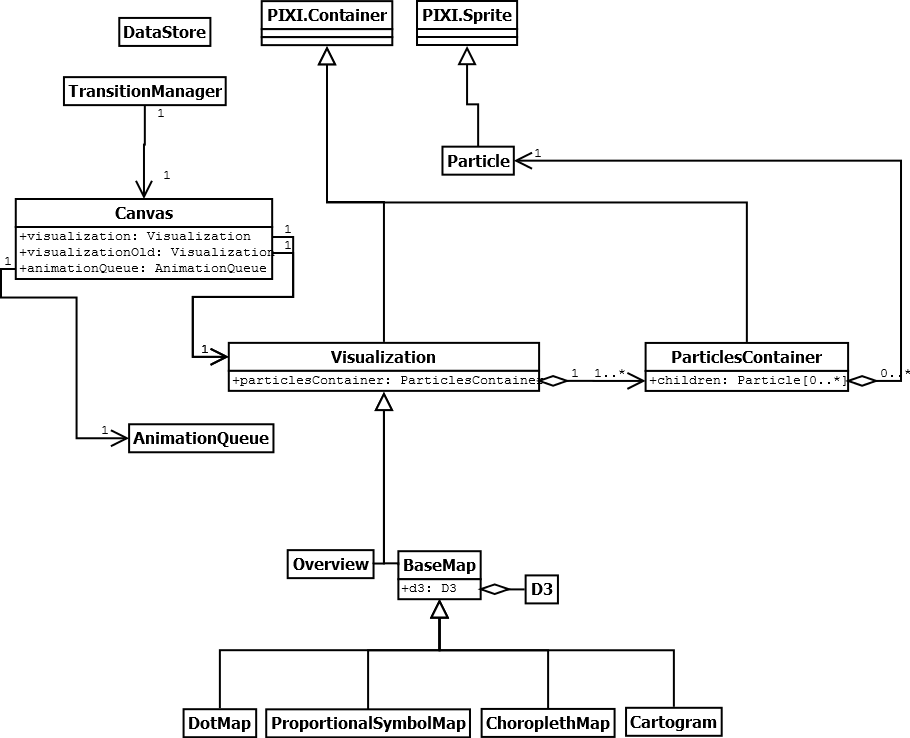
\includegraphics[width=0.8\textwidth,keepaspectratio]{images/results/dia.png}
\caption[
    Overview of the application architecture in the form of a class diagram.
]{Overview of the application architecture in the form of a class diagram.}
\label{fig:uml-practical-approach}
\end{figure}
%TC:endignore

\begin{description}
\item[DataStore] \hfill \\
An object of the DataStore-class is used to load the SuperStore-Sale dataset. In addition to initally loading it, it also parses and analyses the dataset. Each attribute of the dataset got classified to handle the attributes correctly later on. For the sake of convenience, three different classification types were used: numeric, date, nominal and unknown.

\item[PIXI.Container] \hfill \\
\ac{Pixi} features functionalities like container classes. \textit{PIXI.Container} is such a class and can be used to put objects in it, and scale or move those objects according to the base-canvas.

\item[AnimationQueue] \hfill \\
If an animation is assigned to particles, it is stored in the \textit{AnimationQueue}. This allows to create multiple canvas-based animations and process them sequential.

\item[Canvas] \hfill \\
This class is one of the main classes inside the application. It is needed to not compare it with an HTML-Canvas object. However, this class is responsible for creating the base-canvas of the web-application. Furthermore, it is used to change and update the visual appearance if any interaction happens. A key part of the canvas class is the render function shown in listing \ref{lst:canvas-render} on page \pageref{lst:canvas-render}. It starts off with calling the same function again as soon as possible. The caller-function \textit{requestAnimationFrame} ensures, that the next frame will only be shown if enough resources of the browser are available. Afterwards, all particles and visualisations are animated if something changed. The last line of the listing shows the \ac{Pixi}-renderer. Listing \ref{lst:canvas-autodecet-renderer} on page \pageref{lst:canvas-autodecet-renderer} shows its creation. It features the main canvas-size, background transparency, antialiasing and a lot of other options.

%TC:ignore
\begin{lstlisting}[language=JavaScript, caption={Render function of the canvas class.}, label={lst:canvas-render}]
    render() {
      this.requestFrameID = requestAnimationFrame(this.render.bind(this));

      let areParticlesAnimating = this.particlesContainer.nextStep();
      let isNewVisualizationAnimating = this.visualization.nextStep();
      let isOldVisualizationAnimating =  ? this.visualizationOld.nextStep() : false;

      if (!areParticlesAnimating && !isOldVisualizationAnimating &&
        !isNewVisualizationAnimating && this.animationQueue.length > 0) {

        this.animationQueue.pop()();
        this.particlesContainer.startAnimation();
        this.visualization.startAnimation();
        if (this.visualizationOld){
            this.visualizationOld.startAnimation();
        }
      }
      this.renderer.render(this.stage);
    }
\end{lstlisting}

\begin{lstlisting}[language=JavaScript, caption={Pixi's autodetect-renderer.}, label={lst:canvas-autodecet-renderer}]
    this.renderer = PIXI.autoDetectRenderer(this.width, this.height, {
        transparent: true,
        clearBeforeRender: true,
        antialias: true
    });
    document.body.appendChild(this.renderer.view);
\end{lstlisting}
%TC:endignore

\item[Visualization] \hfill \\
This class is the starting point and the parent class for all other types of visualisations. It stores a reference to the \textit{ParticleContainer} and provides functionality to move, scale or change visualisations.

\item[Overview] \hfill \\
Creating an instance of \textit{Overview} will show all data items as unit-based grid.

\item[D3] \hfill \\
This class is mainly used to wrap all functionality of the \ac{D3} library. It features functions like initialising the base-map as a \ac{SVG} and loading the needed TopoJSON data accordingly. \ac{D3} offers multiple projections for GeoJSON data. Listing \ref{lst:d3-map-init} on page \pageref{lst:d3-map-init} shows a part of the map initialisation with the projection used. The projection is an extension of an Albers equal-area projection discussed in chapter \ref{s:map-projections} on page \pageref{s:albers-equal-area-projection}. It is a United-States-centric composite projection. The lower forty-eight states of america are projected using the default Albers-equal-area projection. However, Alaska and Hawaii use a separate conic equal-area projection. The scale of Alaska is furthermore diminished. It is projected at $0.35\times$ its true relative area. The scale and translation of the map are set to use the available window space and center the map on the screen.

%TC:ignore
\begin{lstlisting}[language=JavaScript, caption={Map initialisation with a map projection, scale, and translation.}, label={lst:d3-map-init}]
    this.projection = this._d3.geo.albersUsa()
        .scale(width)
        .translate([this.width / 2, this.height / 2]);
\end{lstlisting}
%TC:endignore

Another key part of this class is featured in listing \ref{lst:d3-topojson} on page \pageref{lst:d3-topojson}. It shows how TopoJSON is used on the client. The filter function passed to the first \textit{TopoJSON.mesh}-function specifies that only internal state borders should be drawn. Thus, coastlines will not be drawn to retain detail around small islands and inlets. The filter function passed to the second \textit{TopoJSON.mesh}-function extends the first one by only drawing each county boundary once. Thus, if two counties share the same border, it is only drawn once.

%TC:ignore
\begin{lstlisting}[language=JavaScript, caption={TopoJSON usage on the client with the adaption of merging all geographic information.}, label={lst:d3-topojson}]
    this.data.topojson.states = topojson.mesh(
        this.data.us,
        this.data.us.objects.states,
        (a, b) => {
            return a !== b;
        }
    );

    this.data.topojson.counties = topojson.mesh(
        this.data.us,
        this.data.us.objects.counties,
        (a, b) => {
            return (
                a !== b &&
                !(this.getCountyIdentifier(a) / 1000 ^ this.getCountyIdentifier(b) / 1000)
            );
        }
    );
\end{lstlisting}
%TC:endignore

Another important aspect of the \ac{D3} class is the \textit{calculateCentroids}-function shown in listing \ref{lst:d3-calculate-centroids} on page \pageref{lst:d3-calculate-centroids}. It calculates a look-up dictionary for the given level of detail for each data item. Thus, providing a huge performance boost when finding out the centroid of a unit later on.

%TC:ignore
\begin{lstlisting}[language=JavaScript, caption={Calculate a look-up dictionary for all data items depending on the level of detail.}, label={lst:d3-calculate-centroids}]
    calculateCentroids(levelOfDetail){
        const boundaries = this._topojson.feature(
            this.data.us,
            this.data.us.objects[levelOfDetail]
        ).features;

        this.centroids[levelOfDetail] = {};
        for(let boundary of boundaries){
            this.centroids[levelOfDetail][boundary.id] = this.path.centroid(boundary);
        }
    }
\end{lstlisting}
%TC:endignore

% SYMBOL SCALE AND COLOR SCALE TO SHOW

\item[BaseMap] \hfill \\
This is the second class inheriting from the \textit{Visualization} class. It features a single object of the \ac{D3} class. Therefore, it is possible that all deriving classes share the same object of \ac{D3} and thus, all its features and settings. Changing the level of detail of the \textit{BaseMap} will affect the map initialised in \textit{\ac{D3}} and hence, all deriving classes are using the same base-map again. This class is mainly used to share the same object of \ac{D3} for all children.
The decision if the upcoming map should be animated or not handles each subclass on its own. All of them use the same concept of determining the type of transition: each implemented subclass has some kind of \textit{draw}-function which accepts an optional parameter called \textit{animationCb}. If this parameter exists and is not \textit{undefined}, the transition to the upcoming visualisation is animated.
All subclasses based on aggregation are implemented and animated with \ac{D3}. Therefore, dot map is slightly different than these in the terms of structure and usage. Furthermore, all thematic maps based on aggregation are implemented with the method of using a static file consisting of all information. However, the aggregated values could also be calculated every time.

\item[DotMap] \hfill \\
The \textit{DotMap} class is the first one to show data on the base-map. It does not use the \ac{DOM} to create the units on the map. It uses the already existing particles from the particle container inherited from the \textit{Visualization} class. Key part of this class is the determination of animating particles or not.
The herein before mentioned decision if particle should be animated or not is shown in listing \ref{lst:dot-draw-animated} on page \pageref{lst:dot-draw-animated}. It also shows the further executed actions if they should be animated, like projecting the longitude and latitude of the point onto the map and calling the main \textit{draw}-function for each particle.

%TC:ignore
\begin{lstlisting}[language=JavaScript, caption={Particles on a dot map getting animated.}, label={lst:dot-draw-animated}]
    if(this.isFunction(animationCb)){
        for(let particle of this.particles){
            point = [particle.data.Longitude, particle.data.Latitude];
            point = this.baseMap.projection(point);
            particle.coords = point;

            setTimeout(drawFunc.bind(this), 250, particle, this.size);
        }
    }
\end{lstlisting}
%TC:endignore

\item[ProportionalSymbolMap] \hfill \\
Drawing proportional symbols is done by using \ac{D3}. First of all, it does not use the SuperStore-Sale file as a basis, and instead uses the preprocessed TopoJSON file. The \textit{draw}-function of this class gets two parameters: the level of detail which should be drawn and the decision if the symbols should be animated. Listing \ref{lst:psm-draw} on page \pageref{lst:psm-draw} shows how each circle for the proportional symbol map is drawn and eventually animated. Line 8-13 loads the already existing data into the created \ac{SVG}-element. It is important to sort the data first because if this would not happen, bigger circles would cover smaller ones. Drawing the bigger ones first results in zero overpainting. The \textit{.data()}-function returns an array. Iterating through every item in the array is done with the \textit{.enter()}-method. Line 15 and onwards create a proportional symbol called \textit{circle} for each data item in the array. They set its position with \textit{transform} and decide, if its radius should be animated or not.

%TC:ignore
\begin{lstlisting}[language=JavaScript, caption={The draw-function of the ProportionalSymbolMap-class}, label={lst:psm-draw}]
    draw(id, animationCb){
        let map = this.baseMap;

        this[id] = map.svg.append("g")
        .attr("id", `psm-${id}`)
        .attr("class", "bubble")
        .selectAll("circle")
        .data(
            map._topojson.feature(map.data.us, map.data.us.objects[id]).features
            .sort(function(a, b) {
                return (b.properties.orders || 0) - (a.properties.orders || 0);
            })
        )
        .enter()
        .append("circle")
        .attr("transform", function(d) {
            let coords = map.path.centroid(d);
            if(isNaN(coords[0]) || isNaN(coords[1])) return;
            return "translate(" + coords + ")";
        });

        if(this.isFunction(animationCb)){
            this[id]
            .attr("r", 0)
            .transition()
            .delay(300)
            .attr("r", function(d) {
                return map.symbolScale(d.properties.orders) || 0;
            })
            .each("end", animationCb);
        } else {
            this[id]
            .attr("r", function(d) {
                return map.symbolScale(d.properties.orders) || 0;
            });
        }
    }
\end{lstlisting}
%TC:endignore

\item[ChoroplethMap] \hfill \\
The implementation of this type of thematic map is a classified choropleth map. As all the other versions of aggregated thematic maps, the distinction between animated and static drawing is done. Listing \ref{lst:choropleth-part-draw} on page \pageref{lst:choropleth-part-draw} shows a small part of the \textit{draw}-function. If the \texit{animationCb} is truthy, all enumeration units are first coloured with a light grey, followed by a colour transition based on the orders of the unit.

%TC:ignore
\begin{lstlisting}[language=JavaScript, caption={The draw-function of the ProportionalSymbolMap-class}, label={lst:choropleth-part-draw}]
    if(this.isFunction(animationCb)){
        this[id]
        .attr("fill", "#D3D3D3")
        .transition()
        .delay(300)
        .duration(1000)
        .attr("fill", d => {
            let scaled = map.colorScale(
                map.symbolScale(Number(d.properties.orders) || 0) || 0
            );
            return this.getColor[scaled];
        })
        .each("end", animationCb);
    } else {
        this[id]
        .attr("fill", d => {
            let scaled = map.colorScale(
                map.symbolScale(Number(d.properties.orders) || 0) || 0
            );
            return this.getColor[scaled];
        });
    }
\end{lstlisting}
%TC:endignore


\item[Cartogram] \hfill \\
The web-application implements a specific type of cartogram: a pseudo Demers cartogram. A true Demers cartogram would need links between adjacent features. However, the type of cartogram implemented tries to preserve locality instead of connectedness. Therefore, each square is located as close as possible to its origin without overlapping. In order to deliver this kind of information to the user, a collision detection with gravity is used to animate the position of each square. Listing \ref{lst:cartogram-part-draw} on page \pageref{lst:cartogram-part-draw} shows a small part of the \textit{draw}-function. It covers the part of initially drawing each square and afterwards starting the collision detection and the gravity.

%TC:ignore
\begin{lstlisting}[language=JavaScript, caption={The draw-function of the pseudo Demers Cartogramm-class}, label={lst:cartogram-part-draw}]
    this.node = map.svg.append("g")
    .attr("id", `cartogram-${id}`)
    .selectAll("rect")
    .data(this.nodes)
    .enter()
    .append("rect")
    .attr("class", "rect");

    if(this.isFunction(animationCb)){
        this.node
        .attr('width', 0)
        .attr('height', 0)
        .transition()
        .delay(300)
        .attr("x", d => { return d.x - d.r; })
        .attr("y", d => { return d.y - d.r; })
        .attr("width", d => { return d.r * 2; })
        .attr("height", d => { return d.r * 2; })
        .each("end", () => {
            animationCb();

            force
            .nodes(this.nodes)
            .on("tick", this.tick.bind(this, 0.00599))
            .start();

        });
        this[id] = this.node;
    }
\end{lstlisting}
%TC:endignore

\item[ParticlesContainer] \hfill \\
This container contains all particles and ensures, that they are animated in the desired order. Furthermore, it controls the speed of each animated particle.

\item[Particle] \hfill \\
A particle is inherits the functionality of \textit{PIXI.Graphics} and contains information about its position, alpha value, and the data it represents. It exposes methods to draw a particle onto the map and to animate it.

\end{description}

% As one can see, all thematic maps based on aggregation keep a reference of the data shown. Therefore, changing the level of detail first checks, if the map needs to be updated or not.

\subsubsection{Interaction}
% transition
% level of detail
% changing visual appearance

\subsection{User study}
To answer the research question of this thesis, a user study yielding qualitative results was conducted. Such a study verifies that the implemented application fulfills its design goals.
The study setup was held in a laboratory environment with 14 participants. It was necessary that each participant does not know the purpose of proportional symbol maps, choropleth maps and cartograms. This requirement ensures that recognition of the animated transition between two visualisations is not combined with previous knowledge about the thematic map type.

The design of the conducted study was within-subject with think-aloud tasks and a post-task interview. Its primary objective was to check if participants understand the relationship between different geo-spatial visualisations and also help them to extract strengths and weaknesses of each visualisation type. To achieve this, the task participants had to solve was of minor importance. It consisted of finding one of the areas in the United States with the most orders normalised by population. Participants had to justify their answer with the chosen map type. Although, each implemented type of map would be sufficient to answer the question, another requirement was introduced. Participants had to look at every map type at least once. The justification of their answer lead to a post-task interview, where they were asked why they did or did not choose a specific type of map. The participants had to name the advantages and disadvantages of each thematic map if possible (as shown in Chapter \ref{s:univariate-maps} on page \pageref{s:univariate-maps}).
To conclude the study, they had to rate the usefulness of the transitions on a scale from 1 to 5 where 1 denotes the transition as unhelpful and 5 as helpful. Hence, the results of the user study are in a binary format - either a participant could name a particular advantage or disadvantage or not and include a score for the transition overall.

The conducted user study was performed with six female and eight male participants. They were between 21 and 47 years old. They all described themselves as technically affine with some experience in the domain of information visualisation and no experience with transitions between visualisations. The residual chapter shows the results from the study.

Revealing a general pattern of a distribution is the main objective of a dot map. 10 out of 14 participants could name the purpose of this thematic map. Even more participants (11 out of 14) said that it is not possible to determine exact quantities in a dot map due to underestimation of high density areas.

The major drawback of a proportional symbol map was detected by 10 out of 14 attendees. According to their feedback, the east coast of the United States was very hard to read due to close locations with high population and therefore overlapping symbols. However, only six people found that the estimation of quantities is less tedious. Seven people were able to name the advantage of a non-existing areal bias.

Finding hot spots was identified by 100\% of the participants as the primary goal of a choropleth map. Furthermore, nine attendees could also name the areal bias as a disadvantage of a choropleth map.

The distortions a cartogram comes along with are identified by 12 attendees as the main weakness of this type of map. Nonetheless, three participants discovered that cartograms emphasise the attribute mapped to the size of the symbol and eliminate visual biases due to their abstractness.

In addition, 10 participants rated the transition between the thematic maps with a score between three and five. The mean score of the transition is 3,21.


\section{Discussion}
\label{s:discussion}
\cbstart
This Chapter discusses the concept used for animated transitions between geo-spatial visualisations, as well as the evaluation and implementation of the concept.
The first Section of this Chapter deals with the concept of this thesis and its limitations. An abstract analysis with the framework provided by \citeauthor{Munzner2014} is made. The findings of the conducted user study their limitations created by the study design are also part of the first Section. The second part presents strengths and weaknesses of the implemented application. Therefore, each Section provides answers of the derived research question.
\cbend

\subsection{Conceptual Discussion and Conceptual Limitations}
% marc fragen, was hier noch stehen soll
% \subsubsection{Analysis-Framework}
The implemented web application is based on two datasets: a tabular dataset (SuperStore-Sale) and a geo-spatial one (boundaries). These datasets are statically preprocessed and used. This information already answers the question of what the application visualises.

\cbstart
Furthermore, the main objective of the visualisations is to consume information, according to Figure \ref{fig:why} on page \pageref{fig:why}. In addition, users of the application should discover previously unkown knowledge. Considering the performed user study and its task, a user should discover an area in the United States which has the most orders normalized by population.
\cbend

Overall, the application uses static encodings like colour, size and shapes for the different types of maps and motion when changing the visual appearance. This already leads to the possibilities in manipulation. Changing the level of detail, colour scheme and particle speed allow for exploring different settings. However, reducing or changing the displayed information is not possible at all. The implemented types of maps have very specific characteristics, making a consistent aggregation or filtering of information impracticable.


\newpage
\subsection{Technical Discussion and Technical Limitations}
The web application consists of two main parts: the first one is the data acquisition and preparation and the second one is the transition manager handling the animation. The first subsection will discuss the restrictions, advantages and disadvantages coming along with the implementation. This discussion is followed by pointing out the strengths and weaknesses of using the transition manager. The discussion is concluded with an analysis of the used technology.

\subsubsection{Data Acquisition and Data Preparation}
Automatic data acquisition and preparation with GNU-Make is very powerful and flexible. The primal strength of it is that writing a \textit{Makefile} creates a machine-readable documentation for the whole workflow. Recording each step in the process enables reproducibility later on.
Thinking of GNU-Make as a dependency graph is key. Unlike a linear and sequential script, a dependency graph is more modular. For example, a \textit{Makefile} is augmentable with deriving multiple data files from the same zip archive without repeating the download of the archive. Thus, using GNU-Make fulfills already two requirements: it scales very well if using multiple data files from different data sources is desired and modularity is provided with the ability of defining tasks for different concerns. However, one major weakness of GNU-Make is its syntax and possible complexity. Putting the facts into comparison, the advantages outweigh the disadvantages.

The primary setup of pre-calculating every needed information has one major advantage as well as one disadvantage. The client-side web application needs to deliver the file to the client with all information only once. Afterwards, everything can be used without dynamically calculating values. On the one side, the initial loading time of the application is significantly higher compared to only delivering the boundary informations. On the other hand, the acquisition and calculation of data later yields to performance drops whenever the data is needed.
A significant drawback using this setup is that showing additional information to an aggregated symbol is not possible. A thematic map based on aggregation fully relys on the preprocessed dataset. Therefore, showing additional information on the dot-map would make use of the Superstore-Sale dataset with all information accessible, whereas showing additional information for symbols or units in aggregated thematic maps depends on the preprocessed boundary file. From an abstract point of view, the practical implementation uses two different source files for showing one phenomenon, yielding to inconsistency when allowing interaction with the visualisation. Changing the visual appearance also changes their base-data and therefore consistency in interaction concepts is not possible and therefore left out.

\subsubsection{Transition Manager}
The implemented transition manager is a key part of the practical application. It specifies some kind of structure to all visualisation classes. Each step of a transition needs to be implemented in the actual class and the manager only calls the exposed functions in the correct order to create the animated transition. This concept ensures separation of concerns of each exposed function and therefore guaranteeing modularity in creating animated transitions.

The transition table \ref{tab:transition-table} on page \pageref{tab:transition-table} mentions shape transitions which are not yet implemented. This is due to the GeoJSON file acquired from the census bureau. Every enumeration unit is specified as a multipolygon. The GeoJSON specification defines multipolygons as a collection of polygons and polygons as an array of coordinates. However, a polygon can contain multiple rings. If this is the case, the first ring must be the exterior one and any others must be interior rings or holes.
Animating the morphing of an enumeration unit to a symbol would require the starting point to be a polygon in order to create a smooth transition. However, merging the multipolygon of an enumeration unit to a single polygon containing only a single outer ring is not possible. A point in the multipolygon and therefore in the map is unique. This makes it impossible to find the outer ring of multiple polygons.
Another possibility in animated morphing would be to morph each polygon to a particular segment of the symbol. With the current data, the transition will not look smooth. Some polygons in enumeration units are hidden behind the default symbol, therefore an animated morphing of those would look like a random symbol segment appearing without noticing the origin of the polygon.


\subsubsection{Used Technology}
Using ECMAScript6 was not the best choice. Decker presents ECMAScript6 polyfill performance tests. He implements a specific feature with multiple JavaScript versions and compairs their runtime. Furthermore, he uses multiple different transpilers yielding considerable results. The following discussion only includes features which are used in the practical application. It also focuses on the results for Chrome 51, because this is the browser version used for testing the application \iacite{Decker2016}.

His report\footnote{See \href{https://kpdecker.github.io/six-speed/}{https://kpdecker.github.io/six-speed/} for more information.} shows that using classes in combination with babel as a transpiler is $1,8\times$ slower in chrome 51 compared to the default way of creating an object in JavaScript. In addition, using default parameters and calling a parent class with the super keyword is significantly slower. However, the usage of promises is a little bit faster in Chrome 51 \iacite{Decker2016}.

Nonetheless, comparing the used version of JavaScript with its performance with its readability, it is still reasonable because of the better maintainability of the code. Despite its advantage, it is still needed to consider using a different transpiler or JavaScript version if the application should use larger datasets or lacks performance.

\ac{D3} is a proper library providing a huge set of useful functions. Its flexibility and functional style allows code reuse. The usage of this library in the practical application shows no drawbacks at all. Animating all symbols at once or with different timings and applying forces such as gravity is neither a performance problem, nor an implementation problem. However, using \ac{DOM} elements always depends on a proper use of JavaScript. For example, considering a memory leak because of keeping references to deleted \ac{DOM} elements would result in an unresponsive browser.

\ac{Pixi} does not show any disadvantage in the currently implemented application. Displaying particles as sprites is a very scaleable way and animating them with a generalised render function combined with an animation queue provides modularity.


\section{Outlook}
\label{s:outlook}

% wie bereits erwaeht, koennten noch eine menge anderer transitionen implementiert werden wie z.B. jede art von non-inplace transitions, die vl. bessere ergebnisse bringen koennte als die implementierten in-place transitions; hierbei sind der kreativitaet keine grenzen gesetzt



\clearpage
\iheader{References}
\begin{sloppypar}
\printbibliography
\end{sloppypar}


\clearpage
\iheader{List of Figures}
\listoffigures

\clearpage
\iheader{List of Tables}
\listoftables

\clearpage
\iheader{List of Listings}
\lstlistoflistings

